\chapter{Deployment in production} \label{chapter4}

\section{ML models in production}


Rarely do data science projects in academia ever reach production and into a streamlined architecture. There are several reasons which prevent it from happening so. Indeed statistics say that roughly $87\%$ of all data science projects never make it into production \cite{vb2019}.  There are so many issues that hamper companies and developers to do so. We will be discussing only a couple of them here. \par

It is seen that even in professional work environments, data scientists rarely have the access to the right kind of data. Either they face issues due to the \textbf{network policy} in a corporate environment or the data is simply out of their reach. Another issue that quickly catches up with this issue is that a large amount of data already exists in the public domain, however, it is unorganised and exists in a completely unstructured format. More precisely, the data exists in a mixture of various formats namely structured, unstructured and semi-structured data. Such types of data need to go through rigorous cleaning and upkeep mechanisms, the process flow of which is sometimes difficult to figure out. Along with these two issues comes a very humane issue regarding the very basis of how data scientists typically work: in an individual manner. However, putting data models into production happens to be the best example of a collaborative effort by a company and hence can’t be single-handedly attempted by an individual. Apart from that technical issues of choosing the right framework, selecting the appropriate storage setup for your data and models etc. continue to exist.\par

We realise that the problems discussed above are as technical as they are humane. All these requirements gave rise to a completely new role for an MLOPs engineer \cite{Odegua2020}

Fortunately, for this project, the deployment of the data models falls within its current scope. All the ML models which would be trained and tested would be loaded onto the proprietary \textbf{Ezmeral MLOPs platform by HPE}. The servers for the same reside alongside the required hardware resources on SEBI’s internal servers. Doing this (without going into the details) would make the entire process streamlined i.e. the process of uploading videos, and training models on new data as soon as it is available and at the same time would decrease the manual work involved while doing so. As soon as the deployment has been completed, whether for all the NEWS shows or even a few of them, the internal server would be able to serve requests from within the organization domain (POST methods with JSON body) and at the same time would be able to abstract all the complex code and scripts running in the background. Following is an illustration of the complete MLOPs lifecycle which is allowed by (or within) the Ezmeral MLOPs platform.

\begin{figure}[h]
  \centering
  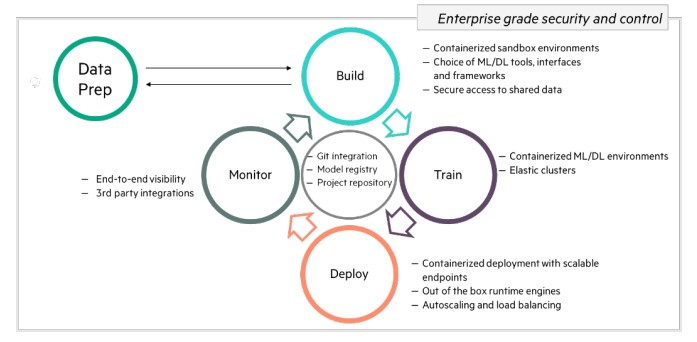
\includegraphics[scale=0.9]{chapter4/ML_DL lifecycle.jpeg}
  \caption{Machine learning lifecycle in production}
  \label{fig:ml_dl_cycle}
\end{figure}

\section{A two-part deployment}

This section deals with the needs of SEBI requiring a two-part deployment and the importance of each type in detail.

\subsection{Ezmeral MLOPs} \label{ezmeral}

The remaining part of this section deals with a proper \textit{yet brief} study of the very exhaustive HPE Ezmeral official documentation to send these models to production. It should be noted that the Ezmeral platform is quite large and only a small part of it deals with proper MLOPs. An even smaller part concerns the project at hand due to the nature of the license procured by the governing organization (SEBI) i.e., we won’t be looking at complicated use cases involving Kubernetes clusters or anything similar. Only the relevant parts of the study have been mentioned below.
The entire Ezmeral architecture looks something as follows. \newpage

\begin{figure}[h]
  \centering
  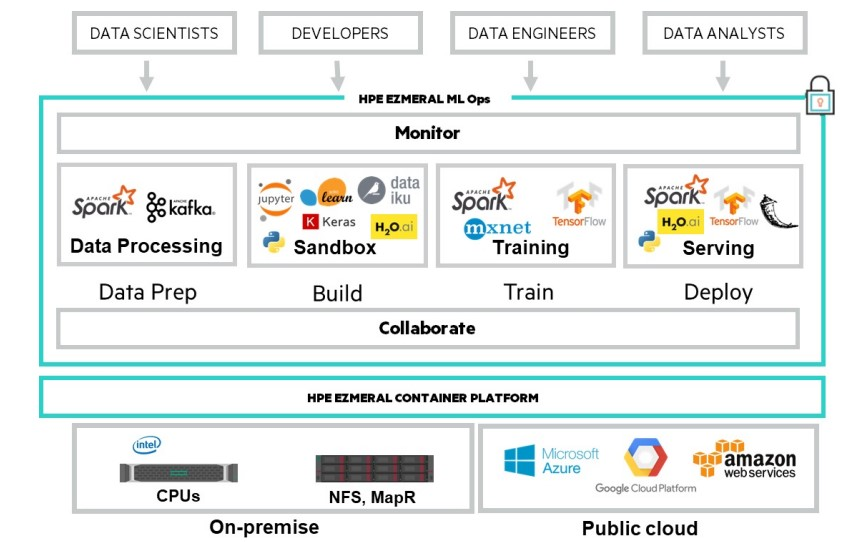
\includegraphics[scale=0.7]{chapter4/ML_DL solution.jpeg}
  \caption{The Ezmeral MLOPs solution}
  \label{fig:ml_dl_sol}
\end{figure}

As per the above architecture following are some sequential steps to be followed while deploying a model to production: \cite{Chiang2020}

\begin{enumerate}
\item Usually, the process begins with the setting up of a proper environment within the Ezmeral cluster. This involves the allocation of appropriate system privileges to various users in a system. Since it’s a server-based system, it is customary to have multiple users and to allocate their various levels of access to the system. The platform admin is responsible for this job. After doing so, various required apps (which are essentially docker images) relevant to the application may be downloaded.
\item After this the project repository is created and appropriate data loaded. This may include pre-written scripts, datasets for training and testing as well as pre-trained models (which may be improvised later on). It should be noted that each one of those things belongs to persistent storage and there would be no data loss in the case of a server outage.
\item Followed by this an appropriate training cluster is to be allocated for a given project: the software concerned currently allows bindings with a variety of CPUs and VCPUs (called flavours). These have different specifications in terms of memory and speed.
\item  This is followed by actual programming in a Jupyter notebook attached to this cluster wherein after the initial phase, dedicated training regimes would utilise these cluster resources.
\item  Followed by the creation and training of a model within the attached Jupyter notebook, the programmer is expected to \textbf{register the model} for further training at a later stage. At this point, the model gets stored in the persistent section of the Ezmeral cluster could be utilised later for further and more advanced training. Beyond this, in typical industrial use cases (such as this), scheduled scripts are just run which re-run this training procedure as many times as required.
\item  After a successful model registry, the server should be in a position to serve requests from the expected domains (in this case only requests from within the SEBI domain). To do so, again appropriate CPUs/VCPUs are assigned to balance the load, serve REST API requests etc.
\item It should be noted that only the scoring script written in Python is run for any given request with the appropriate arguments provided in the JSON request. Hence, apart from the complex steps described above, the entire process boils down to a single Python script execution at the end. \par

\textbf{Followed by this the server is ready to respond to a variety of requests from the concerned domain}.
\end{enumerate}

This concludes the discussion on the entire ML – DL workflow to be used on the Ezmeral MLOPs platform. However, we didn’t go into details about server availability in terms of uptime or downtime nor did we go into the details of the amount of storage available to SEBI who has purchased this platform. It so turns out that although this discussion was not done, this is one of the most principal aspects of the deployment. \par

The Centos VM on top of which the entire Ezmeral cluster resides is used for a lot of tasks \textbf{\textit{apart from the one described above}}. This leads to a low-frequency and high-latency solution which is not good for any MLOPs service use case. Therefore, it was decided that although this setup would be developed in its entirety, this is reserved for only single-usage queries for obtaining the output to only specific videos at a time. \par

The greater requirements at the time were to perform massive batch processing workflows which are freely running and would manage to process several hundreds of videos in sequence. Hence, the second part of the deployment concerns a single VM workflow as described in the following section.

\subsection{Single VM workflow} \label{vm}

To overcome the single-usage and as-in-required constraints described above, we have decided to go for an \textbf{automation script} that calls the main Python script repeatedly to process the bulk of videos that are in turn fetched from a remote server. In this case, it is SEBI’s Datalake server. \par

The concerned setup involves a Linux VM running Centos 8.2 which is relatively ideal and is not involved in unnecessary workflows apart from the concerned one. All the required assets i.e. code (the main Python script \textit{aka} the scoring script in the above section), data (ML models and image templates or masks) and excel files containing a readymade listing of companies are to be made available on the VM. Apart from this the automation script (which is also written in Python) resides on the VM. The logic inside the automation script is segmented into the following parts.

\begin{itemize}
 \item Connecting and disconnecting to the remote server.
 \item Fetching and sending files from and to the remote server respectively.
 \item Performing normal command-line actions on the VM on which it resides: running the Python scoring script repeatedly with command-line arguments and deleting unnecessary files after a single execution run.
 \item Show the current stage of the workflow which is under progress and display a final summary of the total no. of videos that have been processed successfully and(or) the number of videos that have failed.

\end{itemize}

We shall elaborate on the last point a little further. Execution of the scoring script on a single video file leads to the production of a single CSV file at the location of the VM and produces a very large log file wherein the entire output of the script was redirected. The CSV file and the log file need to be sent back to the remote server followed by which they are to be deleted from the VM. Since the video file also doesn’t have any further use, it is also deleted subsequently. The correct order in which this is to be done is elaborated in the last section of this chapter as a guideline for similar scenarios. Upgrades have been planned for this workflow as detailed further in section \ref{future}.


\section{Overall software flow}

\textbf{Step 1}: Open a connection with the remote SEBI Datalake server. Exit the program if a timeout error occurs with an appropriate exit code. \\[5mm]
\textbf{Step 2}: Fetch the next video file in sequence from the remote server. \\[5mm]
\textbf{Step 3}: Run the Python scoring script on the same. This will lead to the production of a log file. And a CSV file only if the execution is successful. \\[5mm]
\textbf{Step 4}: Delete the video file. \\[5mm]
\textbf{Step 5}: Send a copy of the log file to the server and delete its instance from the VM. \\[5mm]
\textbf{Step 6}: If \textbf{Step 3} was successful, send a copy of the generated CSV file to the remote server and delete its instance from the VM.


\end{enumerate}

The entirety of the above process flow has been shown on page \pageref{fig:soft_process_flow}.

\begin{figure}[h]
 \centering
 \begin{tikzpicture}[node distance=2cm]
  \node (start) [startstop] {Start};
  \node (conn) [process, below of=start, yshift=0.5cm] {Open connection with remote server};
  \node (dec1) [decision, below of=conn, yshift=-1.5cm] {Connection timeout?};
  \node (stop1) [startstop, right of=dec1, xshift=3.5cm] {Stop};
  \node (fetch) [process, below of=dec1, yshift=-1.5cm] {Fetch video file from server};
  \node (exec) [process, below of=fetch, yshift=0.5cm] {Execute scoring script};
  \node (del_video) [process, below of=exec, yshift=0.5cm] {Delete video file};
  \node (send_del_log) [process, below of=del_video, yshift=0.5cm] {Send log file to server and delete from VM};
  \node (dec2) [decision, below of=send_del_log, yshift=-1.5cm] {Successful execution?};
  \node (stop2) [startstop, right of=dec2, xshift=3.5cm] {Stop};
  \node (send_del_csv) [process, below of=dec2, yshift=-1.5cm] {Send CSV file to server and delete from VM};
  \node (stop) [startstop, below of=send_del_csv,yshift=0.5cm] {Stop};
  \draw [arrow] (start) -- (conn);
  \draw [arrow] (conn) -- (dec1);
  \draw [arrow] (dec1) -- node[anchor=west] {No} (fetch);
  \draw [arrow] (dec1) -- node[anchor=south] {Yes} (stop1);
  \draw [arrow] (fetch) -- (exec);
  \draw [arrow] (exec) -- (del_video);
  \draw [arrow] (del_video) -- (send_del_log);
  \draw [arrow] (send_del_log) -- (dec2);
  \draw [arrow] (dec2) -- node[anchor=west] {Yes} (send_del_csv);
  \draw [arrow] (dec2) -- node[anchor=south] {No} (stop2);
  \draw [arrow] (send_del_csv) -- (stop);
 \end{tikzpicture}
 \caption{Overall software process flow represented as a simple flowchart}
 \label{fig:soft_process_flow}
\end{figure}



\section{Guidelines for deployment}

This section presents a set of guidelines for the two types of deployment detailed in sections \ref{ezmeral} and \ref{vm}.

\begin{enumerate}
 \item Concentrate on three fundamental aspects of the MLOPs solution namely how the data is going to be stored and retrieved, what frameworks are applicable and(or) available for your job and finally the iterative processes involved in your MLOPs solution \cite{Odegua2020}.

\item Condense your workflow to a few specific data types in which your input data is to be stored e.g. .mp4 files as in this case.

\item Be careful with the amount of data to be stored: look for the best solution fitting your budget.

\item Classify whether you would be dealing with batch workflows or predictions by your ML models in real-time as detailed in sections \ref{vm} and \ref{ezmeral} respectively as this shall greatly affect your outcome.

\item If you are dealing with batch workflows as in section \ref{vm}, the order of fetching and deleting files is paramount. Classify files into input, files produced irrespective of the status of the result and files produced only on successful execution. Order them by size and the sequential points of failure. Delete the largest input file(s) first followed by sequential cycles of sending files to the remote server and deleting them.
